%
% Analysis and forecasting of the Swiss Rent Index
% 1993 to 2018
%
% authors:      Faralli Zully, Spörri Marc
% date-hand-in: 2018-05
%

\documentclass[11pt,a4paper]{article}

% Setup packages
% ------------------------------------------------------------------------

\usepackage[T1]{fontenc}
\usepackage[utf8]{inputenc} 

\usepackage[english]{babel}  % language settings
\usepackage{lmodern}         % font to use
\usepackage{chngcntr}

\usepackage{graphicx}        % use modern graphics formats

\usepackage{amsmath}         % math packages
\usepackage{amssymb}
\usepackage{siunitx}         % takes care of units and errors

\usepackage[round]{natbib}   % bibliography options

\usepackage{xcolor}          % use color names

\usepackage{fullpage}

% hyperref creates links in a pdf, and lets you set pdf options
\usepackage[
    pdfpagelabels,
    plainpages=false,
    pdfauthor={Faralli Zully, Spörri Marc},
    pdftitle={Analysis and forecasting of the Swiss Rent Index 1993 to 2018},
    pdfproducer={},
    pdfcreator={LaTeX2e (pdfLaTeX+Biber/Biblatex on Kile/TexLive/Debian9 and TeXnicCenter/MiKTeX2.9/Windows10)},
    pdfsubject={Analysis and forecasting of the Swiss Rent Index 1993 to 2018},
    pdfkeywords={swiss rent index}
]{hyperref}   % Hyperlinks

% clever refs lets you write \cref{x} instead of \cref{x}
\usepackage[
    %capitalise,   % cap the fig, table... refs
    noabbrev,     % use Figure instead of fig.
    nameinlink    % make the whole thing clickable
]{cleveref}


% Settings
% ------------------------------------------------------------------------

\counterwithin{figure}{section}
\bibliographystyle{apa}      % bibliography style to use
\graphicspath{{graphics/}}   % all graphics are in the graphics folder.
                             % by default, search there!

% document settings
\title{Analysis and forecasting of the Swiss Rent Index, 1993 to 2018}
\author{Faralli Zully, Spörri Marc}
\date{\today}


% My own commands
% ------------------------------------------------------------------------

% note \TODO{} in teh sourcecode to get reminded later that you still have work todo
\newcommand{\TODO}[1]{%
    \textcolor{red}{ %
        \textbf{[ !!!TODO: #1 ]}%
    }%
    \PackageWarning{TODO:}{TODO: #1}%
}


% The actual document
% ------------------------------------------------------------------------
\begin{document}

% title
\maketitle
\newpage

% insert the table of contents
\tableofcontents
\newpage


% ------------------------------------------------------------------------

\section{Introduction}

In this project we analyze the time series of the quarterly collected Swiss rent index from 1993 to 2018.
The main goal of the project is to draw inference from the rent index time series and to predict its future values and a future trend.
In order to do that we do first a transformation of the data in a mean-centered stationary time series by eliminating the trend and possible seasonal components.
Afterwards we are going to model our transformed, stationary data by fitting and testing a set of autoregressive moving average processes (ARMA) in order to select the best candidate model for our transformed, stationary data \cite[p.~82--110]{bd02}.
The selected model will be used to describe and interpret our data as well as to predict future values for the Swiss rent index.


% ------------------------------------------------------------------------

\section{Data Description}

The data is provided by the Swiss Federal Statistical Office, implying 100 quarterly observations of the Swiss rent index beginning by the 2nd quarter of the year 1993 and ending by the first quarter of the year 2018.
The rent index measures the inflation of the rented dwellings in Switzerland.
It is the most significant partial index of the Swiss consumer’s price index, representing a weighted share of 13 percent of this index.

The data are collected quarterly, based upon a stratified random survey sampling of around \num{10000} lessors.
The time series' first observation (2nd quarter of the year 1993) will be the reference value which is set to a base index of 100 and represents the weighted average rent at this time in Switzerland (OFS, 2016: p. 20-23).


% ------------------------------------------------------------------------

\section{Data Analysis}

The first step in any analysis of a time series is to plot the data in order to identify discontinuities or a sudden change of level in the series\cite[p.~23]{bd02}.
As we can see from \cref{fig:indiceloyers_timeseries} there seems to be a clear positive monotonic trend in the time series of the Swiss rent index.
However, the increase seems to be higher in the 1990ies.
It may be advisable to analyse the series by breaking it into two segments \cite[p.~23]{bd02}.
For that purpose we have a look at the segmented plots 1993 to 2009 and 2009 to 2018 (see \cref{fig:indiceloyers_test_train}).

We can see a slightly slower increase in the period from 2009 to 2018 indicating that during the years 1993 to 2009 the growth in rents was faster than in the years after the year 2009.
This fact can be well explained by the big real estate depression in the early 90ies in Switzerland, therefore the time series starting at 1993 is consequently starting from a relatively low initial level and, given the low initial level and the better conjunctural perspectives, the growth  was faster during the 1990ies (irgendwas zitieren 90er jahre depression), whereas from the year 2009 on the growth in rents slowed down, which can be very well explained by the US subprime crises triggered in the year 2008 and followed by a long-lasting global recession \TODO{(zitiere irgendwas)}.

However, they are apparently no outliers, sudden changes or major discontinuities and there is evidently no reason to do further data adjustments or variance-stabilizing transformations like Box-Cox-transformations, for instance {boxcox64}. \TODO{sett hier a ref haere oder wieso isch das boxcox64 in gklammere?}
Therefore we start our work in the next section by transforming our data into a stationary time series \cite[p.~45--82]{bd02}.


% ------------------------------------------------------------------------

\section{Transformation of the Data into a Stationary Time Series}

In this section we want to produce a noise sequence with no apparent deviations from stationarity, meaning we want to transform our data in such a way that covariances between the observations are not depending on time and that we obtain a zero mean expectation and constant variances \cite[pp.~14--23]{bd02}.

However, the objective is not to get a pure white noise sequence  with no dependence among the residuals neither, since there would no further modelling to be done except to estimate their mean-expectation (which would be zero in the centered transformed series) and variance.
The objective is to obtain a stationary series with some few significant dependence among the residuals anyhow, so we can look for a more complex stationary time series model for the noise that accounts for the dependence.
Since dependence means that past observations of the noise sequence can assist in predicting future values this allows us to get a better prediction quality than with a pure white noise sequence \cite[p.~35]{bd02}.

In order to get our noise sequence we have to eliminate any trend and/or seasonal components from our data.
In the next few subsections we will fit several models to get a stationary series.
Afterwards we check our fitted models first for stationarity by tests like the Augmented Dickie-Fuller-Test for the null hypothesis of a unit root (with the alternative hypothesis of stationarity, by consequence \citep{adf}) as well as the Kwiatkowski-Phillips-Schmidt-Shin-Test (KPSS-Test) for the null hypothesis that the observations are trend stationary \citep{kpss92}.

Furthermore we test the estimated noise sequences by examining some simple tests whether or not the obtained residuals are values of independent and identically distributed random variables (as mentioned above: that should not necessarily occur, otherwise we would be confronted with too much randomness in our stationary series and our prediction work would be simply done by estimating mean of the white-noise, which is zero for all predictions $X_{t+1}$, $X_{t+2}$, $X_{t+3}$ etc. in case of a mean-centered stationary series).

In a final step we check them visually by plotting the autocorrelation-function as well as the partial auto-correlation in order to get sure that we are not modelling a white noise sequence on the one hand, and to get an idea of the orders of p and q, respectively for a possible ARMA(p,q)-model, on the other hand \cite[pp.~83--110]{bd02}.
Once we have found a good way to transform our data into a stationary series we will fitting and testing a set of candidate models for our transformed data in \cref{sec:FitTestModel}.

\begin{figure}
    \centering
    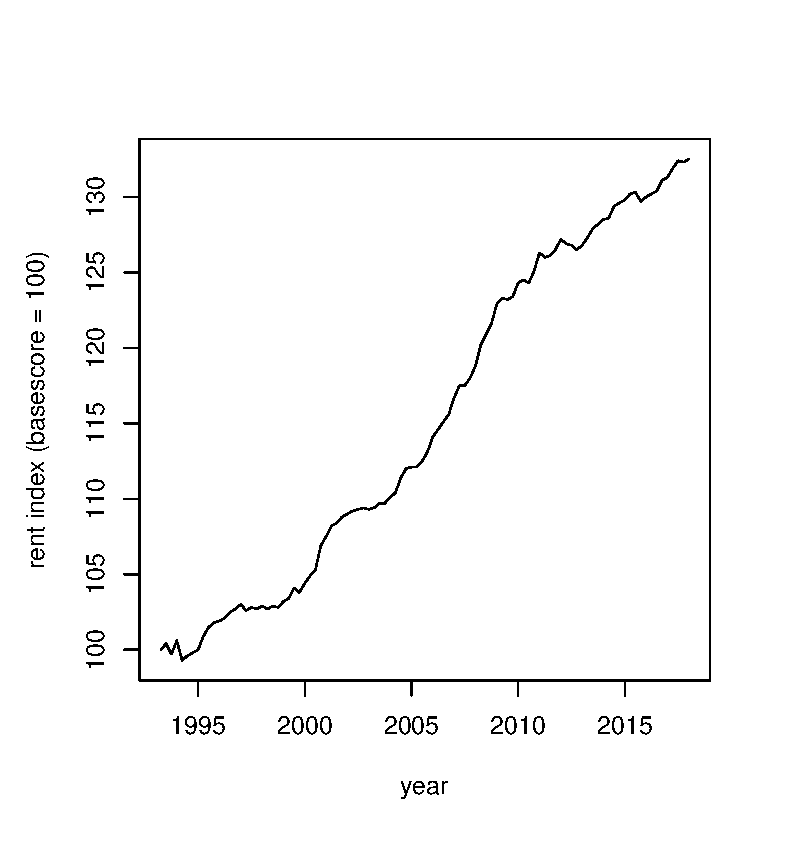
\includegraphics[width=0.7\textwidth]{indiceloyers_timeseries}
    \caption{Swiss rent index, years 1993 to 2018}
    \label{fig:indiceloyers_timeseries}
\end{figure}
 
\begin{figure}
    \centering
    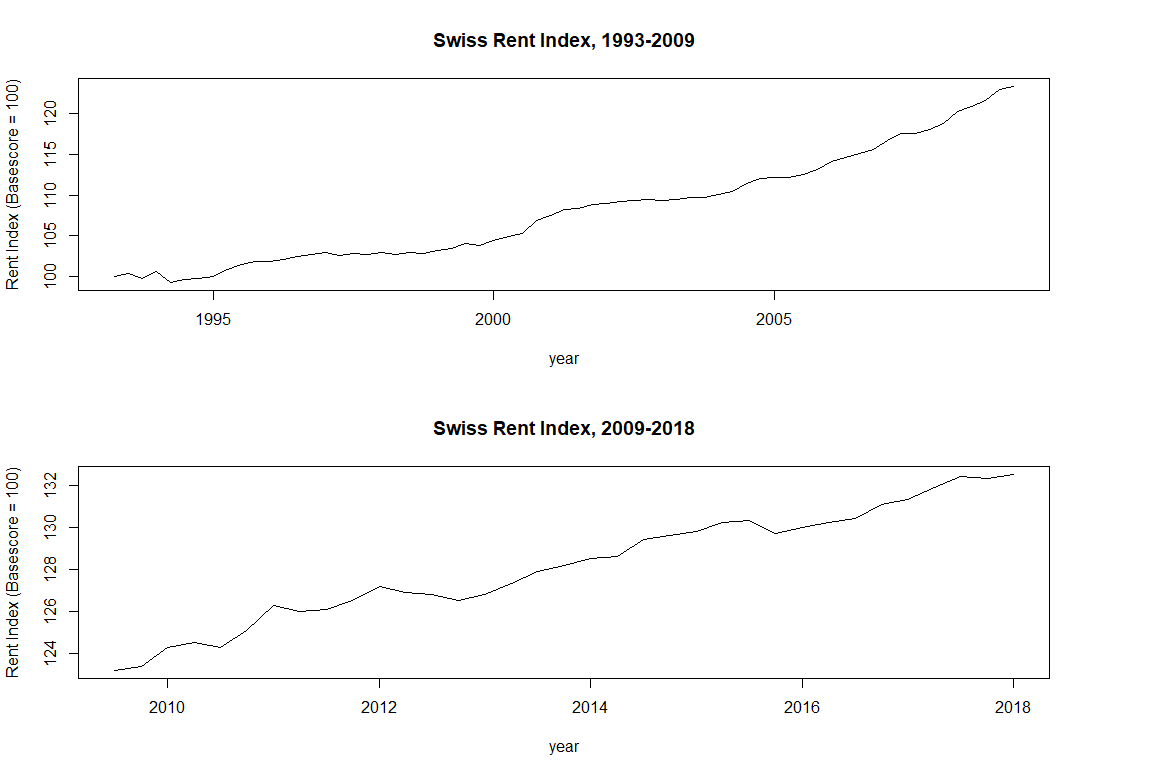
\includegraphics[width=0.8\textwidth]{indiceloyers_test_train}
    \caption{Swiss Rent index, periods from 1993 to 2009 and from 2009 to 2018}
    \label{fig:indiceloyers_test_train}
\end{figure}


\subsection{Method 1: Trend Elimination by fitting polynomial models}

Since the time series \ref{fig:indiceloyers_timeseries} indicates a probable polynomial trend, especially a linear one, we are starting by fitting different polynomial trends by ordinary least squares estimation \cite[p.~11]{htf09}.

We are now modelling a noise sequence (residual time series) by estimating and subtracting a linear, a quadratic, a cubic as well as a logarithmic trend.
The latter  helps to transform a potentially exponential increase in the rent index into a linear trend, even though at first glance the time series \cref{fig:indiceloyers_timeseries} looks more like a linear than an exponential trend, we are going to test for a logarithmic trend either.

The regression models by ordinary least squares estimation \cite[p.~11]{htf09} showed highly significant trend coefficients for all for polynomial models and no significant seasonal effects.\footnote{
    Since the data are collected quarterly we used a linear regression model with d=4 dummy predictors to check for significant seasonal coefficients, meaning a dummy for every quarter.
}

So all of the polynomial models would explain our data extremely well, which is indeed not surprising given the fact that the trend is consistently positive monotonic and therefore highly consistent with other positively monotonic models as our 4 polynomial trend models are (further details on the estimated trend and seasonal coefficients as well as their significance can be found in \cref{fig:summary_cubicmodel} in the tables appendix).\footnote{
    Interpretation of p-values of regression model coefficients are to be handled with care in the case of time series since these models are assuming independence of the observations which hardly never holds true in a time series except white-noise.
    One has to keep in mind that in case of time series we don't want to draw inference on the regression coefficients, our purpose for the regression coefficients is a different one: by looking at their p-value we get an idea whether or not there is a polynomial trend to eliminate in order to get a stationary time series
}

\begin{figure}
    \centering
    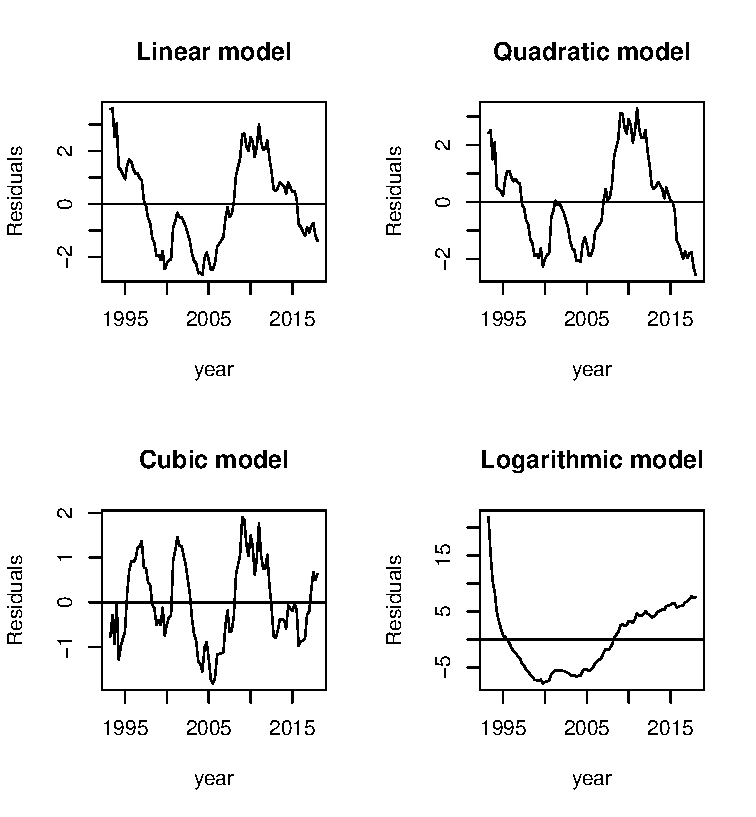
\includegraphics[width=0.8\textwidth]{resid_polynomials}
    \caption{Residuals of the fitted linear, quadratic, cubic and logarithmic model}
    \label{fig:resid_polynomials}
\end{figure}

Nevertheless, even though there is evidently a highly significant polynomial trend in rent index series, that doesn't mean necessarily that its residual time series are stationary.
Unfortunately that happened as we have a look at the four noise sequences in \cref{fig:resid_polynomials}.
The series wanders up and down for quite some periods, meaning that the basic properties of stationary processes, time-independent expectation and constant variance over time are not fullfilled here \cite[p.~49]{bd02}.

This time-dependence is confirmed as well by the sample ACF and PACF.
(cite bd02 zu acf pacf) \cref{fig:acf_pacf_cubicmodel}, exemplified on the cubic model because it was the best-performing polynomial model in terms of the adjusted $R^2$, indicate lot of significant auto-correlations outside the 95-percent-confidence bounds of $+/-1.96/sqrt{n}$.
These bars don't die out quickly and indicate time-dependence and non-stationarity \cite[p.~21]{bd02}.\footnote{
    Similarly strong auto-correlation patterns hold true for the ACF and PACF plots of our other polynomial trend models (linear, quadratic and logarithmic) which will not be shown here.
}


\begin{figure}
    \centering
    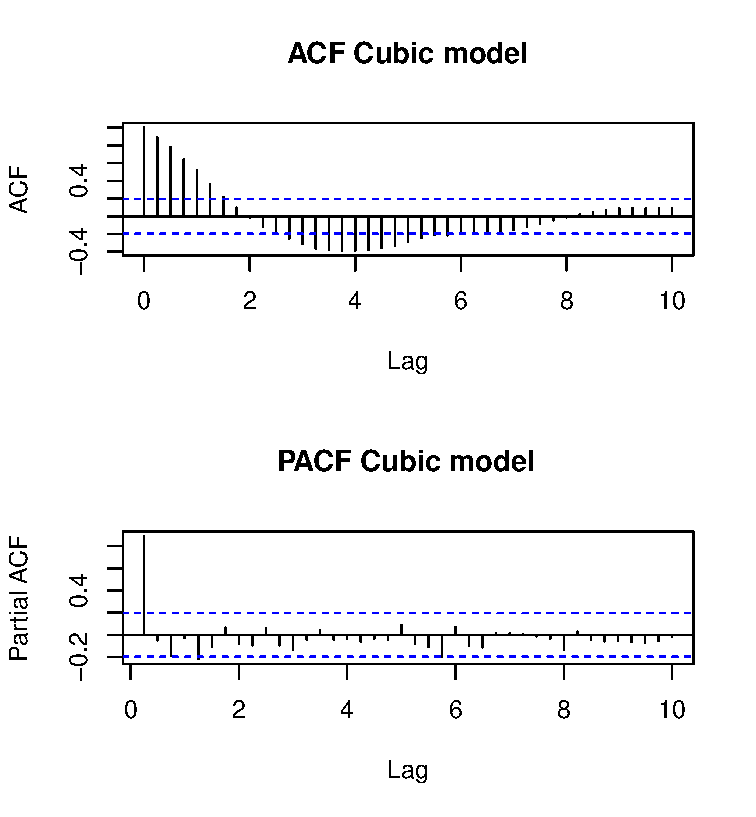
\includegraphics[width=0.6\textwidth]{acf_pacf_cubicmodel}
    \caption{Sample Autocorrelation and Partial autocorrelation function of the Cubic model}
    \label{fig:acf_cubicmodel}
\end{figure}


\subsection{Method 2: Trend elimination by differencing}

Since the fitted polynomial models didn't help to get a stationary time series we will try to eliminate the trend by differencing.
We will differentiate the data at different lags (1, 2, 3 and 4) in order to generate a noise sequence and consequently get a stationary series \citep[p.~35]{bd02}.
Again we will show first the residual plots and testing them afterwards by the sample ACF and PACF as well as the Ljung-Box-, Augmented Dickie-Fuller- and the KPSS-Test.


\subsubsection{Modelling the estimated noise sequences}

\begin{figure}
    \centering
    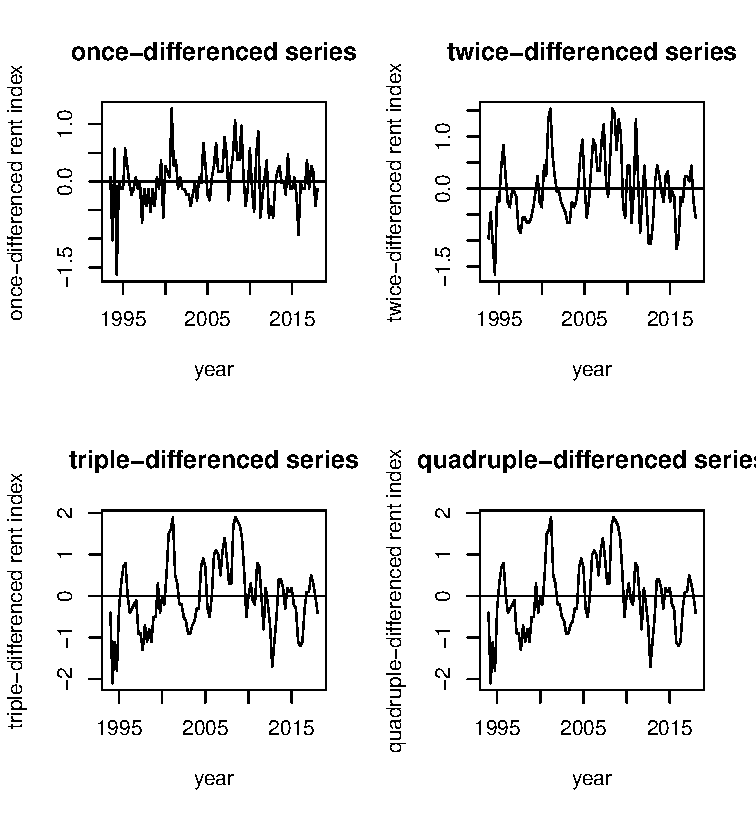
\includegraphics[width=0.8\textwidth]{resid_diff_all}
    \caption{Residuals of the differenced series (1x, 2x, 3x, 4x).}
    \label{fig:resid_diff_all}
\end{figure}

As we can see in the \cref{fig:resid_diff_all} the first two models look already quite promising in contrast to the residual time series above by polynomial trend elimination, showing here obviously time-independent noise sequences with presumably constant expectation and variances.

However, the once-differenced series shows mostly patterns of a white-noise which is not what we intend since in case of a white-noise and too much randomness prediction quality becomes rather poor (Expectation of all the predictions $X_{t+1}$, $X_{t+2}$, $X_{t+3}$ etc. would become zero in case of a mean-centered series).


\subsubsection{Testing the noise sequences}

We are going to test the estimated trends first visually, by looking on the sample autocorrelation-function (ACF) and the sample partial autocorrelation-function (PACF), afterwards we are applying three diagnostic tests for stationarity and independence of the observations, respectively:
The Ljung-Box-Test \citep{LjungBox78} for independence as well as for stationarity the Augmented Dickie-Fuller-Test \citep{adf} and the KPSS-Test \citep{kpss92}.

As we can see in \cref{fig:diff12_acf_pacf}) the white-noise of the once-differenced series is confirmed by the sample ACF where all lags up to 40 fall within the bounds of $+/-1.96/sqrt{n}$ \cite[p.~39]{bd02}.
This underlines that the once-differenced series is to versatile and contains too much randomness in order to do good predictions.

\begin{figure}
    \centering
    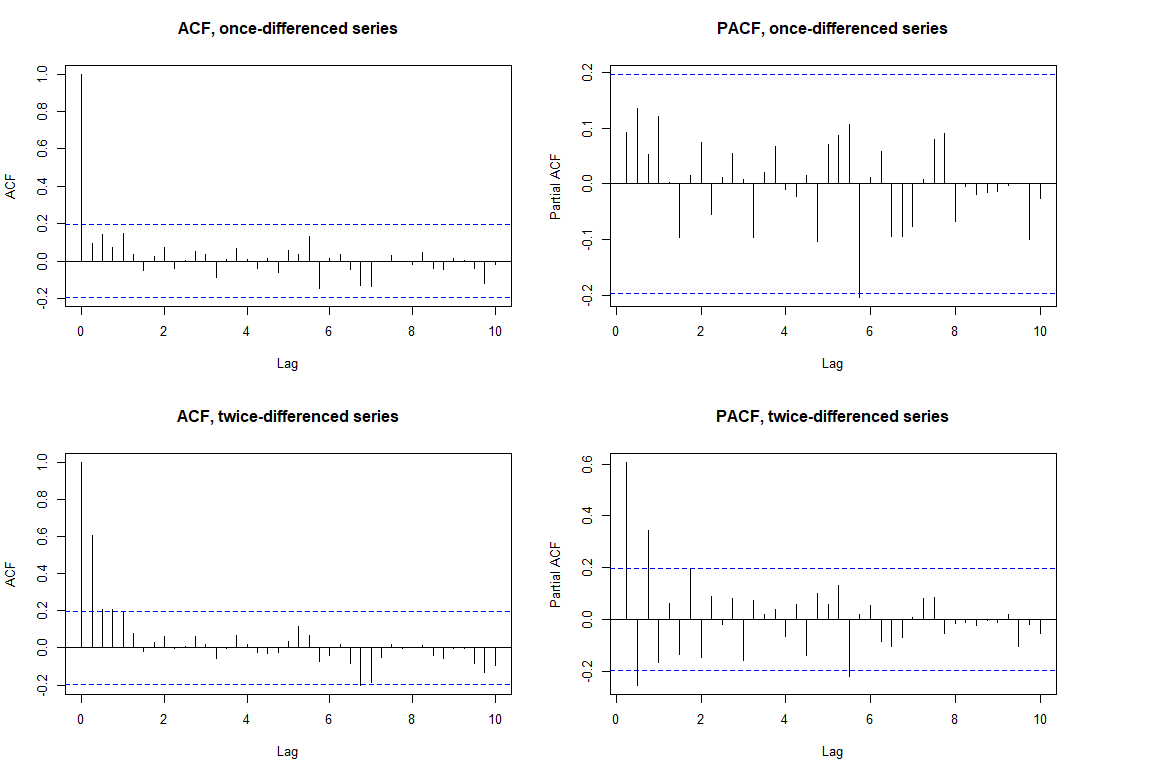
\includegraphics[width=1\textwidth]{diff12_acf_pacf}
    \caption{sample auto-correlation and partial auto-correlation function of the once- and twice-differenced series}
    \label{fig:diff12_acf_pacf}
\end{figure}

In contrast, the sample ACF of the twice-differenced model doesn't indicate a white-noise: there is at least a highly significant correlation at lag 1 and the following three lags are touching the $\pm 1.96 / \sqrt{n}$ - 95percent-confidence-bounds, followed by no more significant bars which die out quickly.
This is a good sign, meaning that on one hand we have at least correlation at lag 1 which is needed to do prediction, on the other hand the covariances seem obviously not too large to be considered time-dependant and therefore we can assume a stationary series here.\footnote{
    Triple- and quadruple-differencing is not appropriate neither.
    Whereas once-differencing is a white-noise, the sample ACF and PACF of the triple- and quadruple-differencing showed significant bars periodically appearing outside the $\pm 1.96 / \sqrt{n}$ - bounds which doesn't allow reliable modelling.
    These plots will not be shown here.
}

From the tests overview in \cref{fig:overview_diffs} we can see for the once-differenced series a p-value of 0.35 for the Ljung-Box-Test.
That was to be expected, meaning that we cannot reject the Hypothesis $H_0$ that there is independence between the observations \citep{LjungBox78} and therefore confirming the white-noise structure in the once-differenced series.

In contrast again, the Ljung-Box-Test for the twice-differenced series rejects the $H_0$ of independence which is a pleasant result giving us the sureness that there is no white-noise in the twice-differenced series.

The Augmented-Dickie-Fuller- and the KPSS-Test suggest for the once- as well as for the twice-differenced trend elimination a stationary time series.
That is a very good result and we can finally conclude to stick with the twice-differentiation in order to transform our data, since the once-differenced series is characterized by too much randomness and white-noise and the triple- and quadruple-differenced series show too large covariances (time-dependence/non-stationarity).
We now center our transformed data by subtracting the mean so that they are prepared fit and test ARMA-models.


% ------------------------------------------------------------------------

\section{Fitting and Testing the Model}
\label{sec:FitTestModel}

\subsection{Order and model selection}

From the sample ACF and PACF (\cref{fig:diff12_acf_pacf}) of our twice-differenced series we can see from the ACF-plot a highly significant spike at the first auto-correlation $\hat{Rho_1}$ and the following bars dying out quickly and lying inside the 95percent-confidence – bounds.
The combined view of the PACF-plot with its exponentially decreasing patterns (in absolute values) and the 1 spike in the ACF-plot let us suggest an MA(1)-model could fit our data quite well.
However, since we are operating with only 100 observations, one can not exclude that there could be underlying exponentially decreasing patterns in the ACF plot as well.
Is this the cse, then exponential decrease (in absolute values) in both ACF and PACF plot would rather suggest an ARMA-model.
Since  we’re are not sure about, we follow a conservative approach and are going to test for MA(1) as well as for ARMA-model(s).
The following matrix (\cref{fig:aicc_matrix}) shows the AICC\footnote{
    The lower the AICC-value the better the model's performance \citep{aic86}.
} for different orders of p and q\footnote{
    p indicates the order of the auto-regressive part and q the order of the moving-average part.
    Its coefficient are generally noted as $phi$ (AR-part) and $theta$ (MA-part).
}.
We can see that an MA(1)-model gives us the lowest AICC-value.
This is as well confirmed by the ACF/PACF plots as evoked above.
However, since the sample ACF and PACF could possibly as well both interpretated as decreasing exponentially (in absolute values), we are going to fit as well an ARMA(1,1) and an ARMA(1,2) model, because they show as well low AICC-values as well (see AICC-Matrix in figure).\footnote{
    Estimations by the autofit()-function of the itsmr R-Packages (cite itsmr) suggest as well an MA(1)-model as best model with a very similar estimate for $\theta_1$ and very close AICC.
    Furthermore ARMA(1,1) and ARMA(1,2) are also suggested by the autofit()-function showing very low AICC-values.
    This can be seen as a succesful robustness check in terms of order selection of p and q.
}

We now estimate coefficients for our three model candidates by the arima()-function (cite arima-package).\footnote{
    The arima-function from the r-package sowieso implies already a preliminary estimation by (hannan rihannen or yule walker) in order go get an initial value for the integrated optimization algorithm:
    the bfgs algorithm (Brockwell, P. J. and Davis, R. A. (1996) Introduction to Time Series and Forecasting. Springer, New York. Sections 3.3 and 8.3.).
    \TODO{reference arima package}
}

\TODO{unit root problem?}

Further evidence for an ARMA(1,2)-model as best candidate model is provided by taking into account an additional MA-term.
We can see then that in an ARMA(1,3) $\hat{\theta}_1$ and $\hat{\theta}_2$ don't differ a lot from the $\hat{\theta}_1$ and $\hat{\theta}_2$ in the ARMA(1,2)-model.
Furthermore $\hat{\theta}_3$ is not significant since it's close to 0 with a large standard error, indicating that the gain by adding a third $\hat{\theta}$- term would be rather poor and ARMA(1,3) would be an overfitted model.
Hence, an moving average of order 2 is sufficient enough.
But we have to note that $\hat{\theta}_1$ and $\hat{\theta}_2$ are rather small compared to their standard errors.
$\hat{\theta}_1$ is only slightly larger than its standard deviation.
$\hat{\theta}_2$ is 2.5 times larger.
However, since we pointed out a unit root issue in the moving average polynomial for the MA(1)- and ARMA(1,1)- models we want to stick with the ARMA(1,2) as our best candidate model, anyhow.
Our final ARMA(p=1,q=2)-process is therefore the following \cite[p.~83]{bd02}:

\begin{align*}
    X_t - \phi_1 X_{t-1} &= Z_t + \theta_1 X_{t-1} + \theta_2 X_{t-2}\\
    &\text{with $t = 1,\dots,n$} \\
    &\text{where ${Z_t} \sim WN(0,\sigma_2)$} \\
    &\text{and the polynomials $(1 - \phi_1 z)$ and $( 1 + \theta_1 z + \theta_2^2 z)$}\\
    &\text{have no common factors.}
    \label{eq:some_equation1}
\end{align*}

\TODO{Formel ueberpruefen! \textasciitilde{} vs $\sim$ vs $\propto$. ist hier in der Formel WN gemeint als: $W \cdot N(x)$ oder $W\!N(x)$}

and the estimated coefficients with the corresponding standard errors (in brackets) are:

\begin{align*}
    \hat{\phi_1}   &= \num{ 0.7974 \pm 0.2055} \\
    \hat{\theta_1} &= \num{ 0.3092 \pm 0.2528} \\
    \hat{\theta_2} &= \num{-0.6685 \pm 0.2583} \\
    \hat{\sigma^2} &= \num{ 0.1793 }
\end{align*}

\TODO{check oeb die darstellig so gwuenscht isch.. mathematisch waers korrekt so..}


\subsection{Diagnostics of the model}

To check the validity of our candidate model we apply as well the following diagnostics:
First, we plot the rescaled residuals and verify that there is not some obvious dependence, trend or else.
We should see a white-noise if the model is valid.
Second, we have a look at the ACF of the rescaled residuals.
Since we are supposed to have a white-noise approximately 95percent of the sample-autocorrelations rhohhat should be inside the bounds $\pm 1.96 / \sqrt{n}$.
\TODO{check this formula: was isch gmeint? $1.96/\sqrt{n}$ oder $1.96\sqrt{n}$}
Third we use the Ljung-Box Test \citep{LjungBox78} to validate that the residuals can be considered as a white-noise by showing p-values for all possible lags \TODO{cite page 5 Lecture notes 11}.

\begin{figure}
    \centering
    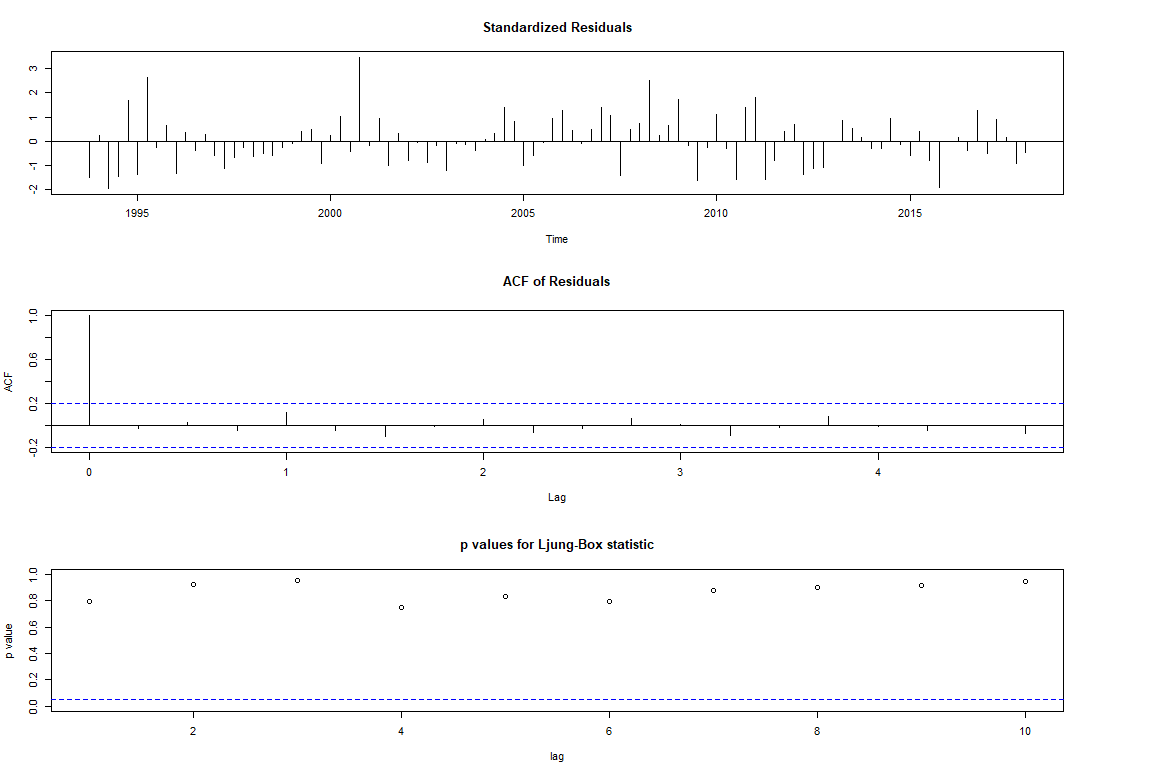
\includegraphics[width=\textwidth]{tsdiag_arma_1_2}
    \caption{ARMA(1,2)-Model: Standardized Residuals, Auto-correlation function of the Residuals and the p-values for the Ljung-Box-Test at each lag}
    \label{fig:tsdiag_arma_1_2}
\end{figure}

We are visualizing these diagnostics by using the tsdiag() function from the ``stats'' R-Package \TODO{cite R Core Team}.
The following \cref{fig:tsdiag_arma_1_2} shows these three diagnostics for each of our model the ARMA(1,2).
We can see that the standardized residuals are supposed to be white-noise in all three cases.
In addition, from the ACF of the rescaled residuals we can see that not a single bar (out of 20) lies outside the bounds bounds $\pm 1.96 / \sqrt{n}$.
And from the Ljung-Box-Tests we can see that the p-value is larger than 5 percent for each lag for each model, meaning that we cannot reject the Hypothesis H0 that these residuals are a white-noise.
So the residuals for all three models seem to be indeed a white-noise, therefore all three models would be valid (good ACF, large p-values on Ljung-Box-Tests) and could be used for forecasting.


% ------------------------------------------------------------------------

\section{Prediction of future values}

In this section we want to predict future values on the base of our fitted ARMA(1,2)-model.
We will do that by first forecasting on our transformed (twice-differenced) series.
Afterwards we will do a retransformation into the initial time series and predict its future values.
In addition, we will give 95 percent confidence bands in case of normally distributed residuals.


\subsection{Forecasting the transformed series}

\begin{figure}
    \centering
    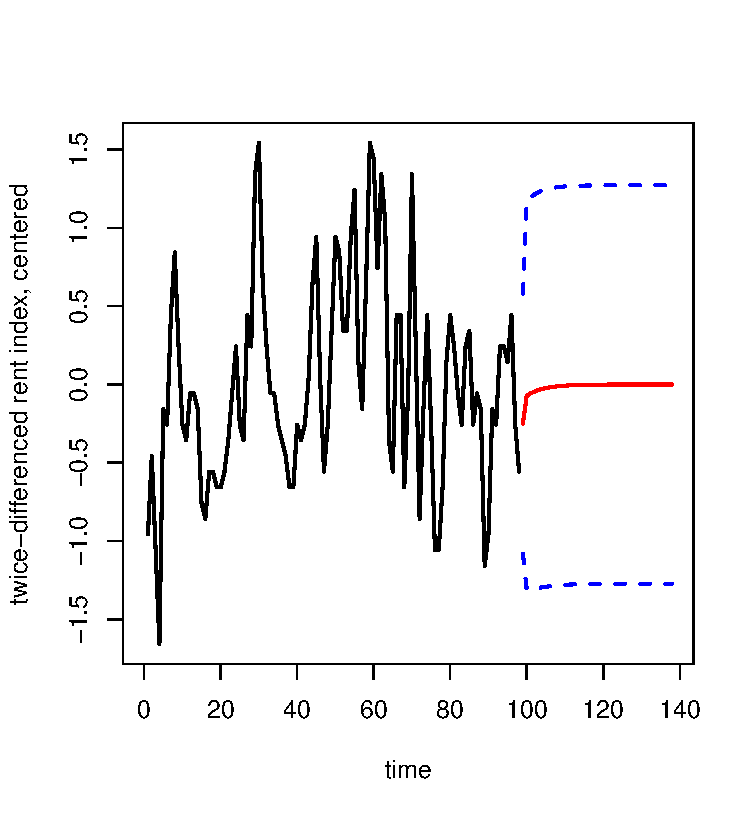
\includegraphics[width=0.5\textwidth]{pred_transformed_series}
    \caption{Prediction and Confidence Bands for the twice-differenced Series}
    \label{fig:pred_transformed_series}
\end{figure}

From \cref{fig:pred_transformed_series} we can see the prediction of a process of adaptation to the zero-mean for the next few quarters.
This is in fact nothing surprising for a mean-centered stationary time series and the smooth positive adaptation process seems to be a reasonable forecast with quite some prediction quality in comparison to a white-noise which would predict directly a zero for the tplus1 observation.
Likewise the quite large 95-percent confidence bands are not that surprising in a strongly differenced series as we have here.
Differenced series like that can contain quite some randomness and result by consequence in large amplitudes as we can very well see.\footnote{
    The indication of confidence bands is weakly justified here since the series’ residuals are successfully tested for normal distribution by the Shapiro-Wilk-Normality Test. \TODO{missing sentence} showed a p-value of 0.07, meaning that the hypothesis H0 of normal distribution can slightly not be rejected \citep{shapiro}.
    However, a quantile-quantile-plot showed patterns of normal distribution for the close-to-mean observations but slightly heavier tails compared to a true normal distribution.
    Therefore interpretations of confidence bands are to be handled with care.
}
However, it would be quite desirable to reduce the variance and by consequence the confidence bands by increasing drastically the number of observations.


\subsection{Forecasting the initial series}

Now that the stationary time series is predicted we need to obtain predictions for the initial time series.
For this purpose we have to consider how we removed the trend and, by consequence, retransform the twice-differenced series into the initial series.

This smooth positively predicted trend goes confirm not only by the long-lasting and consistently increasing trend in the past, but as well with theory about the rent market where expert predict a slight slow-down of the growth in rents but a positive trend still remaining (but less increasing) \TODO{zitiere nzz oder so}.



% ------------------------------------------------------------------------

\section{Discussion}

\TODO{Discuss your results, the strengths and the limitations of your own analysis.}

The difficulty of this project and on the same time is success was to get the data transformed into a stationary process in a way that the residuals don't show too much randomness (white-noise) on the one hand, and on the other hand that we get at least of significant auto-correlations $\hat{Rho}$ anyhow in order to allow predictions based on past observations.
That was not an easy, since the initial time series was strongly monotonically increasing and therefore strongly positively auto-correlated, hence, obtaining a stationary series becomes a hard task:
    first trend elimination by polynomial trend fitting is not possible because of the heavy auto-covariances,
    second once-differencing turned out to be not practicable neither and causing the opposite problems, meaning too much white noise.
But differencing the data twice did the job.
On the same time, the twice-differenced-transformation turned out to contain minor modelling issues since there existed the danger of overdifferencing \cite[~p.194]{bd02}, indicated by the unit root in the moving-average polynomials in case of an MA(1)-model and in the ARMA(1,1) whose estimated theta1 coefficients were on the unit circle or very close to the unit circle.
The problem here lies in the maximum likelihood estimation which possesses properties which chan pose problems for estimation\citep{davidson81}.
When a root of the process is close to the unit circle the asymptotic distribution of the maximum likelihood can be quite inadequate.
However, the estimation by maximum likelihood differ only slightly from other estimations by other methods as  \citep{davisdunsmuir96} have shown.
Therefore our "problematic" estimate of theta close to 1 can still be considered quite accurate.
Furthermore \citep{plosser77} underline that a root close to the unit circle is not that big of a deal as long as the perturbances of overdifferencing are understandable.

To conclude, the choice of the correct data transformation was the dilemma between once-differentiation which leads to a white-noise series which does not allow good prediction, and the twice-differentiation which allows better prediction but suffers possible over-differentiation.
However, our model of choice, the ARMA(1,2) process, does not show unit root problems any more, but its theta coefficients lack of reliability since its standard errors were not that small.
In the context of large variance the relatively small n of 100 observations played an important role here.
Hence, for further predictions on the rent index more data would be desirable.



% ------------------------------------------------------------------------

\section{Conclusion}

\TODO{Conclude the report. Sketch further analyses that you could carry out if you would have more time.}

Further improving work could be done on the transformation into a stationary time series.
Given the fact that the quite promising MA(1)-model (in terms of the ACF and PACF patterns aswell as the AICC) didn't turn out be an ideal choice because of the unit root detected in the moving average polynomial and the consequential danger that excessive use of the difference transformation could induce a non-invertible moving average process \cite[~p.194]{bd02} \citep{plosser77}, one could try a third transformation option: meaning neither fitting a polynomial trend, neither differentiating, but try the Brockwell-Davis-Method \TODO{(cite b d filtering method)} for instance.
Another possibility would be to draw inference in another way, meaning that the estimation of the theta coefficient shouldn't rely only on the maximum likelihood function, but to try alternative estimations like a locally best invariant unbiased (LBIU) approach, for instance \cite{davissong11}.

Last but not least, furthermore improving work could be done during the transformation step by treating the two periods before the subprime crises (year 2009) and after in a different way, since they show slightly different increasing patterns.
One possibility could be, for instance, to try first to logarithmize the stronger increasing data from 1993 to 2009 and afterwards eager for a linear trend elimination or differencing transformation on the total of the data.



% ------------------------------------------------------------------------


\bibliography{bibliography/bibliography}



% ------------------------------------------------------------------------
% ------------------------------------------------------------------------

\appendix

% ------------------------------------------------------------------------

\section{Tables}

\begin{figure}
    \centering
    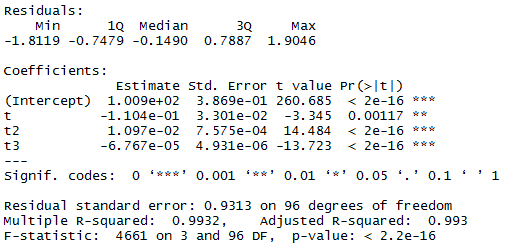
\includegraphics[width=0.7\textwidth]{summary_cubicmodel}
    \caption{summary statistics of the fitted cubic model}
    \label{fig:summary_cubicmodel}
\end{figure}

\begin{figure}
    \centering
    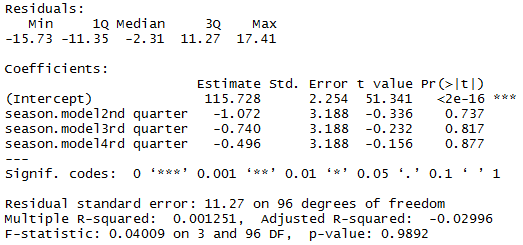
\includegraphics[width=0.7\textwidth]{summary_seasonmodel}
    \caption{summary statistics of the fitted seasonal model}
    \label{fig:summary_seasonmodel}
\end{figure}


% ------------------------------------------------------------------------

\section{Cross-validation of the twice-differenced series}

Cross-validation with a test data set considering only the last 35 of the 100 observations (see \cref{fig:diff2_testset} above) confirms furthermore the non-stationary character of the twice-differenced-model 
Box.test(d2.indiceloyers.test, lag=2, type="Ljung-Box") p-value of 0.033 suggests the data are (time-)independent
adf.test(d2.indiceloyers.test, alternative = "stationary", k=2)  H0 of non-stationarity cannot be rejected which is not a problem, that could be due to lack of observations
kpss.test(d2.indiceloyers.test)  with a p-value>0.05 the test data seems to be stationary aswell
the data of the first period (1993 to 2009) twice-differenced series show independent observations as well (see \cref{fig:diff2_test_train}), however we can see a slightly slower increase in the segment from 2009 to 2018 indicating that in the years from 1993 to 2009 the growth in rental prices was higher than in the years in the second's segment which begins from 2009. that can be explained by the big baisse in the early 90ies, starting from a lower initial point and better conjunctural perspectives the increase was stronger, whilst from 2009 on the growth in rental prices slowed down, which can be very well explained by the US subprime crises beginning in the year 2008 followed by a long-taking global recession.

\begin{figure}
    \centering
    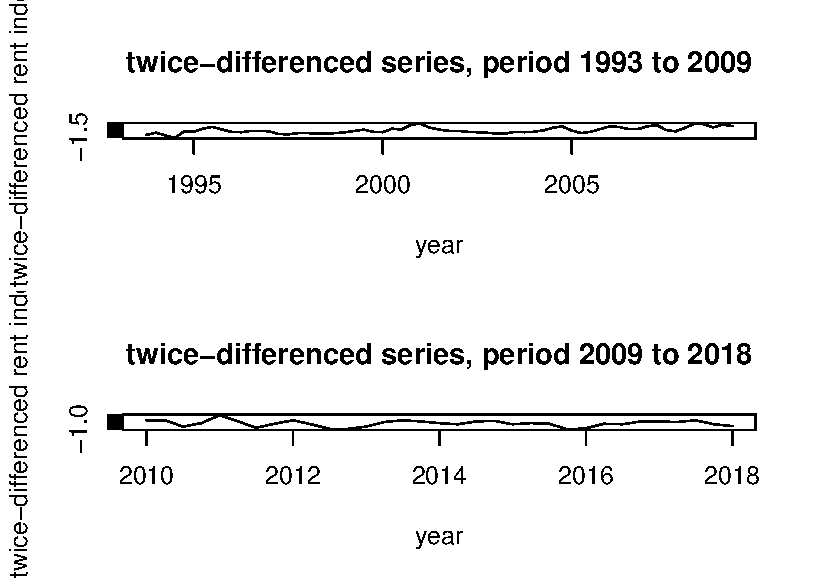
\includegraphics[width=0.8\textwidth]{diff2_test_train}
    \caption{mean-centered twice-differenced series, periods from 1993 to 2009 and 2009 to 2018}
    \label{fig:diff2_test_train}
\end{figure}



\end{document} 
